\chapter{Data Cleaning and Fomatting} \label{chapter:data-cleaning}
%With ST-S being one of the most efficient state-of-the-art skyline algorithms for categorical attributes and in the absence of indexes, the question arises if the algorithm can be further improved. 
In the following, this work presents a novel skyline algorithm called SARTS, which beholds all of the major advantages of the ST-S algorithm, and further improves it by utilizing the more memory-efficient tree structure ART. 

\section{Adaptive Radix Tree} \label{section:art}
The Adaptive Radix Tree (ART) \cite{art} is an efficient indexing structure, specifically designed for main-memory databases. In contrast to most traditional in-memory indexing structures, like binary search trees, ART is able to make optimal usage of modern CPU caches, thus enabling both quicker response times and lower space consumption. The main difference to traditional radix trees is the adaptive resizability of the tree's inner nodes, which results in much more compact tree design. 

\subsection{Characteristics} \label{section:art-characteristics}
%Radix trees have several advantages over comparison based trees, like e.g. binary search trees. The most important ones are: 
%\begin{itemize}
%	\item Better scaling with the number of elements inserted, as the height of the tree depends on key length and not on the number of elements. 
%	\item No extra CPU usage for rebalancing operations is required. 
%	\item Implicit storage of the keys in form of the path taken to the particular element, and thus lower memory consumption. 
%\end{itemize}
The main drawback of radix trees is wasteful space behavior. The reason for this is that all inner nodes in the radix tree have child arrays of exactly the same size, independently of how many of the child pointers are not null. Therefore, if some of the children do not exist, the excessive memory needed to fully allocate the array of pointers is simply wasted. 

The ART tree solves this problem by introducing resizable nodes of four different types: \textit{Node4}, \textit{Node16}, \textit{Node48} and \textit{Node256}. The nodes can have up to 4, 16, 48 and 256 child pointers, respectively. Whenever an inner node has not enough space to insert a new child pointer, it grows to the next bigger type. Similarly, if one of the existing child nodes has been deleted from the tree, then its parent checks if the number of its children is small enough to shrink to the next smaller size. 

\begin{figure}[h]
\centering
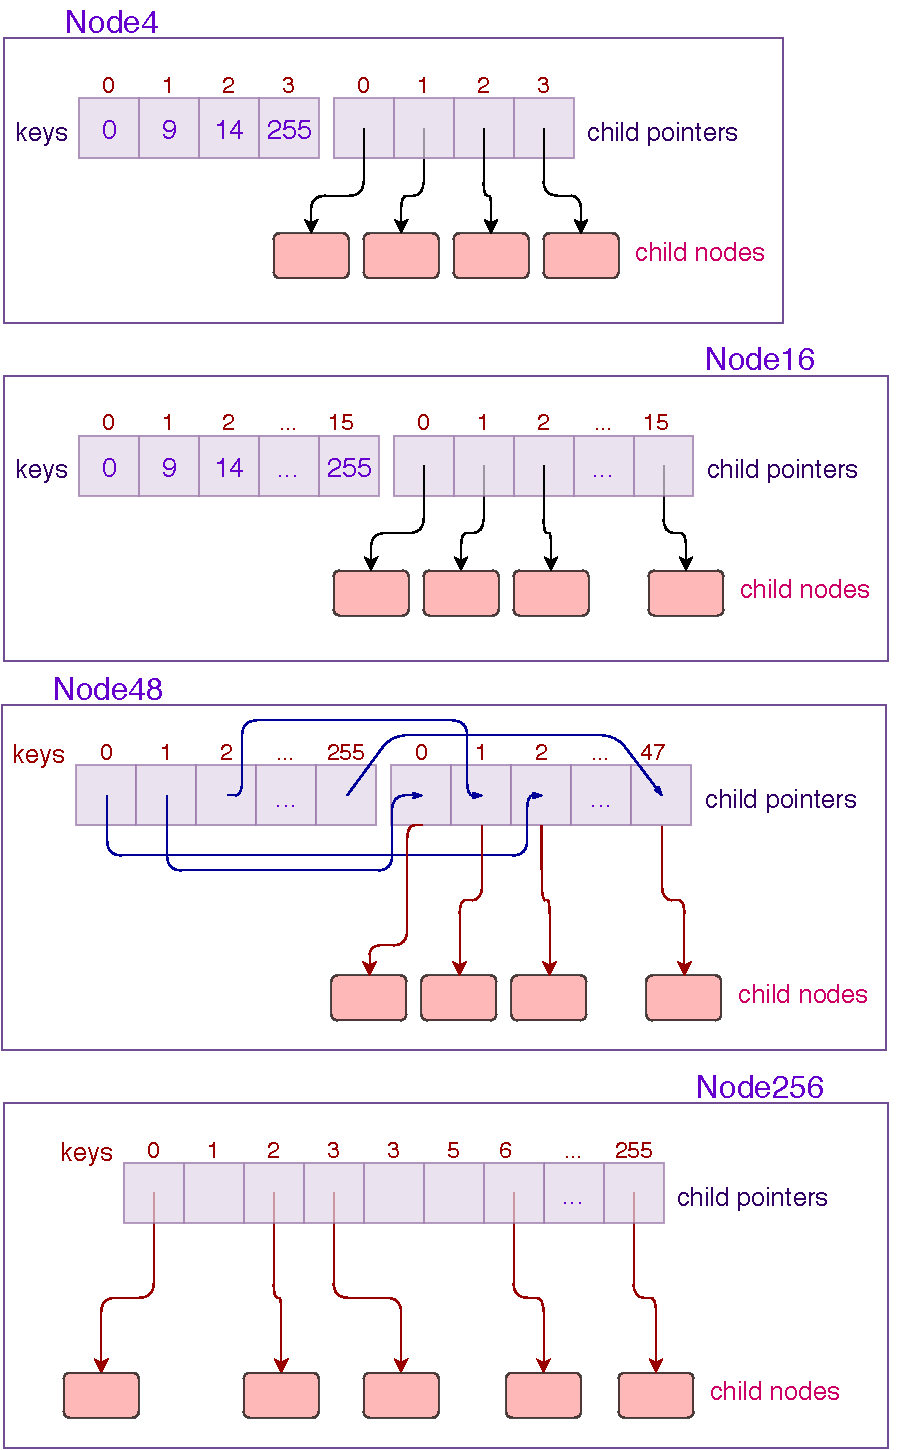
\includegraphics[width=0.8\linewidth]{figures/art-nodes}
\caption{Node Types of the ART Tree}
\label{fig:art-nodes}
\end{figure}

Each of the nodes consists of two different arrays, which function similarly to a key-value store. The entries in the keys array point to the corresponding entries in the array with child pointers. The structure of the four node types is illustrated in Fig.~\ref{fig:art-nodes} and described in the following: 
\begin{itemize}
	\item \textbf{Node4:} The first array is responsible for storing the key bytes in ascending order. The second array holds the pointers to the child nodes. Both arrays are of size 4. 
	\item \textbf{Node16:} This node type is the same as Node4, except for that its arrays are of size 16. 
	\item \textbf{Node48:} With 48 different entries, sequential search for the right entry in the keys array would take too much time. Therefore, Node48 implements a 256-element array for the key entries. Unlike Node4 and Node16, the key bytes now can be found directly in the index of the array, and the elements of the array are pointers to the entries in the children array. 
	\item \textbf{Node256:} This is the largest possible and also the simplest node type in the tree, and can hold up to 256 different entries. It only consists of one array. The key bytes can be found in the index of the array and the entries are child pointers. This way, no indirection is needed in this node type. 
\end{itemize}
In addition to that, each of the nodes possesses a header which holds attributes such as the node type and the number of its chidren. This list of attributes can be adjusted depending on the particular use case of the ART tree. Chapter \ref{section:sarts} makes use of such adjustments. 

Due to the complex structure of the ART nodes, special operations are needed to make use of them. These include \textit{findChild}, \textit{newNode} and \textit{grow}. The operations are explained in greater detail in \cite{art}; the C++ code to each of them can be found in Appendix \ref{appendix-code} to this work. 

%\subsection{Core Algorithms} \label{section:art-algorithms}
%In this section, some of the most important operations that are part of the ART tree are explained. The full C++ code to each of them can be found in the appendix to this work (section \ref{appendix-code}). 
%% Insert
%To begin with \textit{insert}, its main functionality is the following: 
%\begin{enumerate}
%	\item Starting from the root (which is the size of Node4 initially), the first key byte of the new tuple is taken. 
%	\item Depending on the current node type, the corresponding child pointer is found. If the child does not yet exist, then the pointer is null. 
%	\item If the child pointer is null, the node checks if it needs to grow in order to insert a new child. If it has to --- it does, if not --- it does not. The new child is created and a pointer to it is stored in the children array. 
%	\item The edge to the next node is followed. 
%	\item The procedure repeats recursively, until the last byte of the key has been used. At this point, the tuple (and the information within it) is inserted into a leaf node. The key bytes of the tuple do not need to be stored explicitly. 
%\end{enumerate}
%
%% findChild
%\noindent Finding the right child within a node depends on the type of the current node. This is how the \textit{find\_child} function works:
%\begin{itemize}
%	\item \textbf{Node4:} The keys array is traversed until the element is found that corresponds the key byte entry of the given tuple. The index of this element is now the index of the child pointer in the children array. If the pointer is null, then no such child exists yet. In any case, the child pointer is returned. Both arrays are traversed sequentially as the array size is too small to require more efficient searching techniques. 
%	\item \textbf{Node16:} The keys array of Node16 is bigger than that of Node4. Therefore, it is sensible to utilize some faster searching technique than simply traversing the array from left to right. The authors in \cite{art} propose to either use binary search or SIMD\footnote{Single Instruction, Multiple Data} instructions to speed up the search. As soon as the index of the given key byte is found, the child pointer under this index can be returned, just like in Node4. 
%	\item \textbf{Node48:} The given key byte is taken as the index of the keys array. The element stored under this index is the needed index of the children array. If the element is marked as empty (e.g. with the value 48 in the entry\footnote{The value 48 is vacant, because the keys array of Node48 only holds values between 0 and 47 due to the size of its children array.}), then the function returns a null pointer. Otherwise, the child pointer under this index is returned as the next node. 
%	\item \textbf{Node256:} The given key byte is the index of the needed child entry. The child entry is returned either as a node pointer or a null pointer.  
%\end{itemize}
%
%% newChild
%\noindent Every new child node that is created is always of the smallest-possible Node4 type, because it is empty at the beginning. Creating a new child, however, is still node-type-dependent. The functionality is introduced in the following: 
%\begin{itemize}
%	\item \textbf{Node4 \& Node16:} To find the correct position for the new key entry, the keys array, which is sorted in ascending order, is traversed, until the correct position for the new key byte is found. If this position is already taken, then it is freed by moving all the hindering entries one slot to the right. The same happens with the children array to keep the correct indexing order. Now the new key byte and the new child pointer are added under the same index to the respective arrays. 
%	\item \textbf{Node48:} The new child is added in the first free slot of the children array. Then, a pointer to this slot is saved in the keys array at the index that equals the new key byte. 
%	\item \textbf{Node256:} The new child is simply added at the position with the index that equals the new key byte. 
%\end{itemize}
%
%% grow
%\noindent Growing a node with the \textit{grow} operation is relatively straightforward: 
%\begin{enumerate}
%	\item A new node of the next-bigger type is created. 
%	\item The key bytes, the child pointers as well as any other information stored in the current node are copied into the new node. 
%	\item The parent of the current node gets updated about the new child. Its pointer now points to the new child. 
%	\item The current node is deleted to avoid potential misunderstandings and to free now unused memory. 
%\end{enumerate}

% path compression and lazy expansion
\subsection{Further Optimizations} \label{section:art-further-optimizations}
In addition to the core functionality of ART, the authors propose two further optimizations. The first one is called \textit{lazy expansion}. With this technique, inner nodes are only created if there is more than one path to the leaves passing through them. Otherwise, they are simply left out to save space and to reduce access time to the leaves. The second technique is called \textit{path compression}. It results in removing all inner nodes that only have one child node. %Since the part of the key which was previously stored in preceding inner nodes now misses, some workarounds, such as storing partial key vectors at inner nodes, are necessary to make this technique work. 
Both lazy expansion and path compression could be useful when trying to save even more space and to improve lookup times. More details on both techniques are provided in \cite{art}. 

\section{SARTS - A Novel Skyline Algorithm} \label{section:sarts}
%idea
In the following, SARTS (Skyline using ART Sorting-based), a novel skyline algorithm for categorical attributes is presented. It makes use of the core concepts of ST-S (chapter \ref{subsection:sts}), and further improves it by implementing a more efficient indexing structure for dominance checks --- the ART tree. 

% approach
The interface of the ART tree has been kept similar to that of the N-Tree in ST-S. This enables for a very straightforward integration of the ART tree into the algorithm, because the \textit{insert} and \textit{is\_dominated} operations still have the same signature as in ST-S. While \textit{insert} is slightly different from the original variant on the inside, the \textit{is\_dominated} operation is almost identical to the one in ST-S. Therefore, for the pseudo-code of SARTS and \textit{is\_dominated} it can be referred to Algorithms \ref{alg:sts} and \ref{alg:sts-is-dominated}. 

% pseudocode insert
The \textit{insert} operation for SARTS differs from the ST-S variant in that both finding the correct child to the current node and creating a new child are outsourced into two separate functions: \textit{findChild()} and \textit{newChild()}. In addition to that, before a new child can be created, the current node might first need to \textit{grow()} to the next-bigger type, in order to create space for the new child. The pseudo-code to the \textit{insert} operation is given in Algorithm \ref{alg:sarts-insert}.
\begin{algorithm}[h]
	\caption{INSERT Operation for SARTS} \label{alg:sarts-insert}
	\begin{algorithmic}[1]		
		\State \textbf{Input :} Tuple $t$, Node $parent$ Node $current$, Level $level$, Attributes $atts$
		\If {$level$ = 0}
			\State $node.minScore \gets 0$
			\State $node.maxScore \gets \sum_{i~=~0}^{t.size~-~1}(2^{t.size~-~i}~*~max(atts))$
		\Else 
			\State $node.minScore \gets \sum_{i~=~0}^{level~-~1}(2^{t.size~-~i}~*~t[i])$
			\State $node.maxScore \gets node.minScore~+~\sum_{i~=~level}^{t.size~-~1}(2^{t.size~-~i}~*~max(atts))$
		\EndIf
		\If {$level$ = $t.size$} 
			\If {$node.score$ is $None$}
				\State $node.score \gets score(t)$
			\EndIf
			\State Append $t.tupleID$ to $node.tupleIDs$
		\Else
			\State $child \gets findChild$($current$, $t[level]$)
			\If {$child$ is $None$}
				\If {$current.size$ = 4 \textbf{or} $current.size$ = 16 \textbf{or} $current.size$ = 48}
					\State $grow$($parent$, $current$, $t[level~-~1]$)
				\EndIf
%				\Switch {$current.type$}
%					\Case {Node4}
%						\If {$current.size$ = 4}
%							\State $grow$($parent$, $current$, $t[level~-~1]$)
%						\EndIf
%					\EndCase
%					\Case {Node16}
%						\If {$current.size$ = 16}
%							\State $grow$($parent$, $current$, $t[level~-~1]$)
%						\EndIf
%					\EndCase
%					\Case {Node48}
%						\If {$current.size$ = 48}
%							\State $grow$($parent$, $current$, $t[level~-~1]$)
%						\EndIf
%					\EndCase
%				\EndSwitch
				\State $child \gets newChild$($current$, $t[level]$)
			\EndIf
			\State insert($t$, $current$, $child$, $level~+~1$)
		\EndIf
	\end{algorithmic}
\end{algorithm}

% pseudocode is dominated
The main difference within the \textit{is\_dominated} operation is, similarly to \textit{insert}, the usage of the \textit{findChild()} function any time the correct child for further traversing of the tree needs to be found. 

In addition to that, just like the nodes of the N-Tree, the inner nodes of the ART tree have to be extended by a \textit{minScore} and a \textit{maxScore}, and the leaf nodes by the \textit{score} attribute and an array of \textit{tupleIDs}. This enables faster traversing of the tree during dominance checks by skipping tree regions that cannot dominate the current tuple. 

% The ART version taken
The ART version used in this paper is the basic one for simplicity purposes. It does not incorporate the two optimization approaches \textit{path compression} and \textit{lazy expansion}. 

